\section{Methodology} 

For ring detection, we use the circular Hough Transform (CHT).  Since the
defocued ... method, ring edges are thick, fuzzy and have rather low contrast
against the background.  we have skipped the edge detection, apply HT directly
to the input image, following contrast adjustment.  As a result, the HT votes
are contaminated by pixels that does not belong to any shape and are therefore
very noisy. For the purpose of efficiently and reliably sepearte the signal
from noises, we used a likelihood ratio function to filter the votes.  And
later for determining the ring sizes, radical histogram algorithm is used.

\subsection{Pre-processing}
we apply a contrast adjustment, remove background noise would help.
from histogram background noise gaussian distribution, signal in tail
we find the position and width of the histogram peak, and remove all pixels below threadshold
$$s = I_{\mathrm{peak}} + n *\sigma_\mathrm{peak}$$
n is a parameter, which is usally set to 1.

\subsection{Hough Transform: ring templates} 

Circular Hough transform, maps the input image into accumulator space, x, y and
r.  Although the space is continous, in practice it is divided into discrete
cells.  Each cell corrsponds to superpositions of all ring shapes from postions
included in the cell.  We can view the CHT as a approach combining template
matching and HT. We use ring template with various ring size, covolve with
input image. The covolution is used as votes in accumulator space.

We have studied the impacts of ring templates on the voting. For a step fucntion,
..., side slobes. Therefore we use a skewed function..., ..... To account for the
fuzzy egeds, we gaussain shape of the skewed function,...

\subsection{Likelihood ratio}
Hough transform.
common strategy is to apply an edge detection before HT.
Images of micro particles are fuzzy, does not have a crisp edges. 
Signals can be very close to the background.
We imporve the contrast to gain higher SNR instead of edge detection.

\begin{figure}
\centering
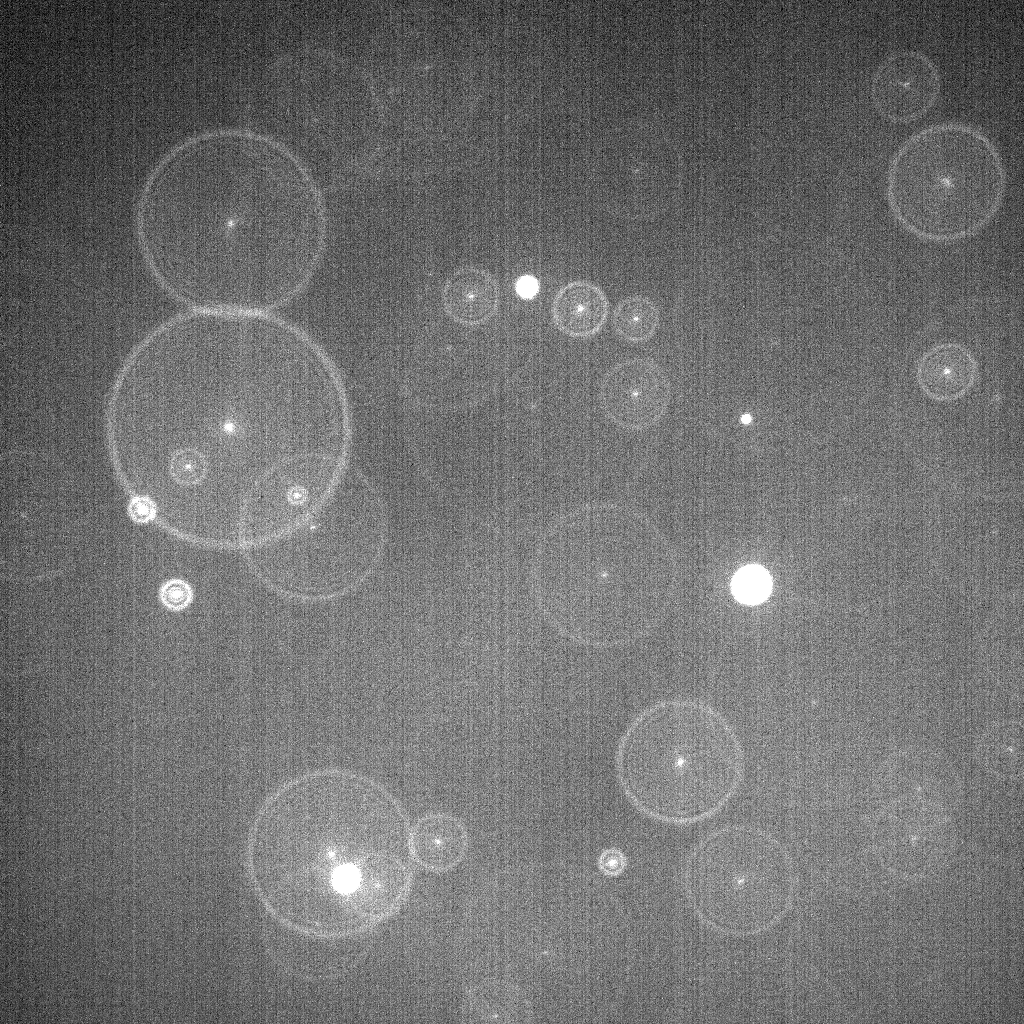
\includegraphics[width=0.35\textwidth]{figs/image1.png}\qquad
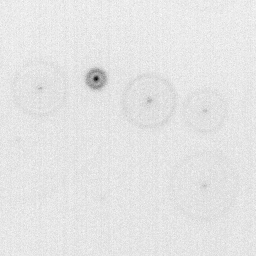
\includegraphics[width=0.35\textwidth]{figs/img0-crop.png}
\label{fig:input}
\caption{Picture captured in experiment.}
\end{figure}


contrast, histogram, singmoid, background fitting

\begin{figure}
\centering
\includegraphics[width=0.25\textwidth]{./figs/img0-crop-contrast.png}
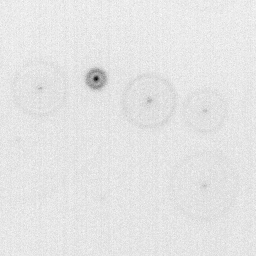
\includegraphics[width=0.35\textwidth]{figs/img0-crop.png}
\end{figure}


Likelyhood function. 
\begin{equation}
    L(\pi_{ij}) = \exp\left( -\frac{1}{\sigma_n^2 } \sum \right)
\end{equation}

